
\documentclass[10 pt,usenames,dvipsnames, oneside]{article}
\usepackage{../../modelo-fracoes}
\graphicspath{{../../../Figuras/licao03/}}


\begin{document}

\begin{center}
  \begin{minipage}[l]{3cm}
\includegraphics[width=2cm]{../../../Figuras/logo}       
\end{minipage}\hfill
\begin{minipage}[r]{.8\textwidth}
 {\Large \scshape Atividade: Nível da caixa d'água}  
\end{minipage}
\end{center}
\vspace{.2cm}

\ifdefined\prof
%Caixa do Para o Professor
\begin{goals}
%Objetivos específicos
\begin{enumerate}
    \item Reconhecer a representação de frações na reta numérica a partir da graduação em uma escala linear.
    \item Associar,  na reta numérica, o segmento unitário à unidade.
    \item Reconhecer a representação de frações do segmento unitário na reta numérica.
\end{enumerate}

\tcblower

%Orientações e sugestões
\begin{itemize}
\item Espera-se que os alunos (i) associem o 0 (zero) à caixa d'água vazia e o 1 (um) à caixa cheia; (ii) Descartem as faixas (c) e (d) porque não respeitam a equipartição e que (iii) reconheçam que as faixas a), b) e e) são marcações possíveis. Discuta com os alunos as vantagens e as desvantagens dessas marcações. A faixa a) traz a marcação da fração $\frac{1}{2}$ associada ao segmento e não ao ponto, o que dificulta a indicação de alturas intermediárias, como $\frac{1}{4}$, por exemplo. A faixa (e) tem poucas marcações, limitando a medição.
\item A atividade aborda a medição de volume a partir de uma escala linear. Os alunos precisam reconhecer que a quantidade de água no recipiente está associada à altura do líquido no recipiente. Para garantir que os alunos compreendam o processo, considere mostrar a eles um recipiente transparente na forma de um paralelepípedo ou de um cilindro e fazer perguntas como ``até onde eu preciso encher para alcançar metade da capacidade? E um quinto?''.
\item Observe que o formato da caixa, um paralelepípedo, possibilita uma escala linear para a medida do volume (o mesmo valeria para um cilindro, por exemplo). No entanto, para outros formatos de caixa, esse mesmo tipo de escala não seria adequado. É o caso, por exemplo, de um cone. Uma tal discussão foge aos objetivos do estudo de frações.
\end{itemize}
\end{goals}

\bigskip
\begin{center}
{\large \scshape Atividade}
\end{center}
\fi

Os quadrinhos a seguir mostram uma caixa-d'água sendo enchida.
Para saber que fração da capacidade da caixa-d'água já está com água, será usada uma faixa graduada para indicar o nível de água na caixa.

\begin{table}[H]
\centering
\setlength\tabulinesep{10pt}
\begin{tabu} to \textwidth{|c|c|}
\hline

\begin{tikzpicture}[scale=2, x=1cm, y=1cm]



\draw [fill=brown] (-.3,0,0) -- (1.3,0,0) -- (1.3,0,1) -- (-.3,0,1) -- cycle;
\draw [fill=brown!70!black] (1.3,0,-0) -- (1.3,-.05,0) -- (1.3,-.05,1) -- (1.3,0,1);
\draw [fill=brown!70!black] (1.3,0,1) -- (1.3,-.05,1) -- (-.3,-.05,1) -- (-.3,0,1);



\draw (0,0,0) -- (1,0,0) -- (1,0,1) -- (0,0,1) -- cycle;

\draw (0,0,0) -- (0,1,0);
\draw [fill=white, opacity=.7] (0,1,0) -- (1,1,0) -- (1,1,1) -- (0,1,1) -- cycle;
\draw [fill=white, opacity=.7] (0,0,1) -- (1,0,1) -- (1,1,1) -- (0,1,1) -- cycle;

\fill [common!80] (0,.25,0) -- (1,.25,0) -- (1,.25,1) -- (0,.25,1) -- cycle;
\fill [common] (0,0,1) -- (1,0,1) -- (1,.25,1) -- (0,.25,1) -- cycle;
\fill [common] (1,0,0) -- (1,0,1) -- (1,.25,1) -- (1,.25,0) -- cycle;

\draw (1,0,1) -- (1,1,1);
\draw (1,0,0) -- (1,1,0);
\draw (0,0,1) -- (0,1,1);
\draw (1,0,0) -- (1,0,1) -- (0,0,1);

\node at (0.5,-.5,.5) {Momento 1};
\end{tikzpicture}

& 

\begin{tikzpicture}[scale=2, x=1cm, y=1cm]

\draw [fill=brown] (-.3,0,0) -- (1.3,0,0) -- (1.3,0,1) -- (-.3,0,1) -- cycle;
\draw [fill=brown!70!black] (1.3,0,-0) -- (1.3,-.05,0) -- (1.3,-.05,1) -- (1.3,0,1);
\draw [fill=brown!70!black] (1.3,0,1) -- (1.3,-.05,1) -- (-.3,-.05,1) -- (-.3,0,1);



\draw (0,0,0) -- (1,0,0) -- (1,0,1) -- (0,0,1) -- cycle;

\draw (0,0,0) -- (0,1,0);
\draw [fill=white, opacity=.7] (0,1,0) -- (1,1,0) -- (1,1,1) -- (0,1,1) -- cycle;
\draw [fill=white, opacity=.7] (0,0,1) -- (1,0,1) -- (1,1,1) -- (0,1,1) -- cycle;

\fill [common!80] (0,.5,0) -- (1,.5,0) -- (1,.5,1) -- (0,.5,1) -- cycle;
\fill [common] (0,0,1) -- (1,0,1) -- (1,.5,1) -- (0,.5,1) -- cycle;
\fill [common] (1,0,0) -- (1,0,1) -- (1,.5,1) -- (1,.5,0) -- cycle;

\draw (1,0,1) -- (1,1,1);
\draw (1,0,0) -- (1,1,0);
\draw (0,0,1) -- (0,1,1);
\draw (1,0,0) -- (1,0,1) -- (0,0,1);
\draw (0,1,0) -- (1,1,0) -- (1,1,1) -- (0,1,1) -- cycle;

\node at (0.5,-.5,.5) {Momento 2};
\end{tikzpicture} \\

\hline

\begin{tikzpicture}[scale=2, x=1cm, y=1cm]

\draw [fill=brown] (-.3,0,0) -- (1.3,0,0) -- (1.3,0,1) -- (-.3,0,1) -- cycle;
\draw [fill=brown!70!black] (1.3,0,-0) -- (1.3,-.05,0) -- (1.3,-.05,1) -- (1.3,0,1);
\draw [fill=brown!70!black] (1.3,0,1) -- (1.3,-.05,1) -- (-.3,-.05,1) -- (-.3,0,1);



\draw (0,0,0) -- (1,0,0) -- (1,0,1) -- (0,0,1) -- cycle;

\draw (0,0,0) -- (0,1,0);
\draw [fill=white, opacity=.7] (0,1,0) -- (1,1,0) -- (1,1,1) -- (0,1,1) -- cycle;
\draw [fill=white, opacity=.7] (0,0,1) -- (1,0,1) -- (1,1,1) -- (0,1,1) -- cycle;

\fill [common!80] (0,.75,0) -- (1,.75,0) -- (1,.75,1) -- (0,.75,1) -- cycle;
\fill [common] (0,0,1) -- (1,0,1) -- (1,.75,1) -- (0,.75,1) -- cycle;
\fill [common] (1,0,0) -- (1,0,1) -- (1,.75,1) -- (1,.75,0) -- cycle;

\draw (1,0,1) -- (1,1,1);
\draw (1,0,0) -- (1,1,0);
\draw (0,0,1) -- (0,1,1);
\draw (1,0,0) -- (1,0,1) -- (0,0,1);
\draw (0,1,0) -- (1,1,0) -- (1,1,1) -- (0,1,1) -- cycle;

\node at (0.5,-.5,.5) {Momento 3};
\end{tikzpicture}

& 
\begin{tikzpicture}[scale=2, x=1cm, y=1cm]

\draw [fill=brown] (-.3,0,0) -- (1.3,0,0) -- (1.3,0,1) -- (-.3,0,1) -- cycle;
\draw [fill=brown!70!black] (1.3,0,-0) -- (1.3,-.05,0) -- (1.3,-.05,1) -- (1.3,0,1);
\draw [fill=brown!70!black] (1.3,0,1) -- (1.3,-.05,1) -- (-.3,-.05,1) -- (-.3,0,1);



\draw (0,0,0) -- (1,0,0) -- (1,0,1) -- (0,0,1) -- cycle;

\draw (0,0,0) -- (0,1,0);
\draw [fill=white, opacity=.7] (0,1,0) -- (1,1,0) -- (1,1,1) -- (0,1,1) -- cycle;
\draw [fill=white, opacity=.7] (0,0,1) -- (1,0,1) -- (1,1,1) -- (0,1,1) -- cycle;


\fill [common!80] (0,1,0) -- (1,1,0) -- (1,1,1) -- (0,1,1) -- cycle;
\fill [common] (0,0,1) -- (1,0,1) -- (1,1,1) -- (0,1,1) -- cycle;
\fill [common] (1,0,0) -- (1,0,1) -- (1,1,1) -- (1,1,0) -- cycle;

\draw (1,0,1) -- (1,1,1);
\draw (1,0,0) -- (1,1,0);
\draw (0,0,1) -- (0,1,1);
\draw (1,0,0) -- (1,0,1) -- (0,0,1);
\draw (0,1,0) -- (1,1,0) -- (1,1,1) -- (0,1,1) -- cycle;


\node at (0.5,-.5,.5) {Momento 4};
\end{tikzpicture} \\
\hline
\end{tabu}
\end{table}

Escolha, para cada um dos momentos, a graduação que lhe parece mais adequada para registrar a quantidade de água representada em cada uma das imagens. Explique sua escolha.

\begin{enumerate}
\begin{multicols}{2}

\item\adjustbox{valign=t}{
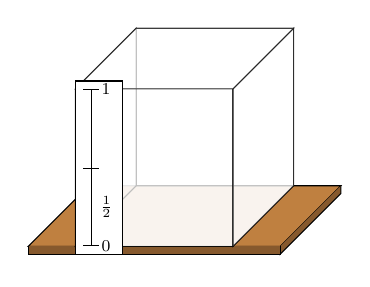
\begin{tikzpicture}[scale=2, x=1cm, y=1cm]

\draw [fill=brown] (-.3,0,0) -- (1.3,0,0) -- (1.3,0,1) -- (-.3,0,1) -- cycle;
\draw [fill=brown!70!black] (1.3,0,-0) -- (1.3,-.05,0) -- (1.3,-.05,1) -- (1.3,0,1);
\draw [fill=brown!70!black] (1.3,0,1) -- (1.3,-.05,1) -- (-.3,-.05,1) -- (-.3,0,1);

\draw [fill=white, opacity=.7] (0,0,0) -- (1,0,0) -- (1,0,1) -- (0,0,1) -- cycle;
\draw [fill=white, opacity=.7] (0,0,0) -- (0,1,0) -- (1,1,0) -- (1,0,0) -- cycle;
\draw [fill=white, opacity=.7] (0,0,0) -- (0,1,0) -- (0,1,1) -- (0,0,1) -- cycle;
\draw [fill=white, opacity=.7] (0,0,1) -- (1,0,1) -- (1,1,1) -- (0,1,1) -- cycle;
\draw [fill=white, opacity=.7] (1,0,0) -- (1,0,1) -- (1,1,1) -- (1,1,0) -- cycle;
\draw [fill=white, opacity=.7] (0,1,0) -- (1,1,0) -- (1,1,1) -- (0,1,1) -- cycle;

\filldraw [fill=white] (0,-.05,1) rectangle (0.3,1.05,1);
\draw [|-|] (.1,0,1) -- (.1,1,1) node [right, scale=.75, xshift=.05cm] {\footnotesize 1} node [ right, pos=0, scale=.75, xshift=.05cm]{\footnotesize 0};
\draw [|-|] (.1,0,1) -- (.1,.5,1) node [right, scale=.75, xshift=.025cm,pos=.5] {\footnotesize $\frac{1}{2}$};

\end{tikzpicture}  
}
\item\adjustbox{valign=t}{
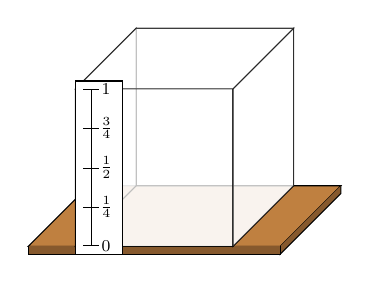
\begin{tikzpicture}[scale=2, x=1cm, y=1cm]

\draw [fill=brown] (-.3,0,0) -- (1.3,0,0) -- (1.3,0,1) -- (-.3,0,1) -- cycle;
\draw [fill=brown!70!black] (1.3,0,-0) -- (1.3,-.05,0) -- (1.3,-.05,1) -- (1.3,0,1);
\draw [fill=brown!70!black] (1.3,0,1) -- (1.3,-.05,1) -- (-.3,-.05,1) -- (-.3,0,1);



\draw [fill=white, opacity=.7] (0,0,0) -- (1,0,0) -- (1,0,1) -- (0,0,1) -- cycle;
\draw [fill=white, opacity=.7] (0,0,0) -- (0,1,0) -- (1,1,0) -- (1,0,0) -- cycle;
\draw [fill=white, opacity=.7] (0,0,0) -- (0,1,0) -- (0,1,1) -- (0,0,1) -- cycle;
\draw [fill=white, opacity=.7] (0,0,1) -- (1,0,1) -- (1,1,1) -- (0,1,1) -- cycle;
\draw [fill=white, opacity=.7] (1,0,0) -- (1,0,1) -- (1,1,1) -- (1,1,0) -- cycle;
\draw [fill=white, opacity=.7] (0,1,0) -- (1,1,0) -- (1,1,1) -- (0,1,1) -- cycle;

\filldraw [fill=white] (0,-.05,1) rectangle (0.3,1.05,1);
\draw [|-|] (.1,0,1) -- (.1,1,1) node [right, scale=.75, xshift=.05cm] {\footnotesize 1} node [ right, pos=0, scale=.75, xshift=.05cm]{\footnotesize 0};
\draw [|-|] (.1,0,1) -- (.1,.5,1) node [right, scale=.75, xshift=.025cm] {\footnotesize $\frac{1}{2}$};
\draw [|-|] (.1,0,1) -- (.1,.25,1) node [right, scale=.75, xshift=.025cm] {\footnotesize $\frac{1}{4}$};
\draw [|-|] (.1,0,1) -- (.1,.75,1) node [right, scale=.75, xshift=.025cm] { \footnotesize $\frac{3}{4}$};


\end{tikzpicture}  
}
\end{multicols}

\begin{multicols}{2}
\item\adjustbox{valign=t}{
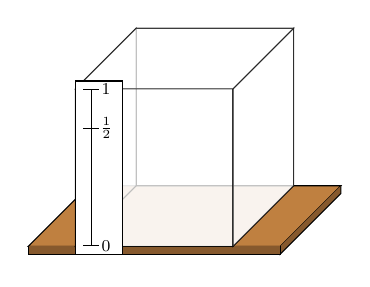
\begin{tikzpicture}[scale=2, x=1cm, y=1cm]

\draw [fill=brown] (-.3,0,0) -- (1.3,0,0) -- (1.3,0,1) -- (-.3,0,1) -- cycle;
\draw [fill=brown!70!black] (1.3,0,-0) -- (1.3,-.05,0) -- (1.3,-.05,1) -- (1.3,0,1);
\draw [fill=brown!70!black] (1.3,0,1) -- (1.3,-.05,1) -- (-.3,-.05,1) -- (-.3,0,1);



\draw [fill=white, opacity=.7] (0,0,0) -- (1,0,0) -- (1,0,1) -- (0,0,1) -- cycle;
\draw [fill=white, opacity=.7] (0,0,0) -- (0,1,0) -- (1,1,0) -- (1,0,0) -- cycle;
\draw [fill=white, opacity=.7] (0,0,0) -- (0,1,0) -- (0,1,1) -- (0,0,1) -- cycle;
\draw [fill=white, opacity=.7] (0,0,1) -- (1,0,1) -- (1,1,1) -- (0,1,1) -- cycle;
\draw [fill=white, opacity=.7] (1,0,0) -- (1,0,1) -- (1,1,1) -- (1,1,0) -- cycle;
\draw [fill=white, opacity=.7] (0,1,0) -- (1,1,0) -- (1,1,1) -- (0,1,1) -- cycle;

\filldraw [fill=white] (0,-.05,1) rectangle (0.3,1.05,1);
\draw [|-|] (.1,0,1) -- (.1,1,1) node [right, scale=.75, xshift=.05cm] {\footnotesize 1} node [ right, pos=0, scale=.75, xshift=.05cm]{\footnotesize 0};

\draw [|-|] (.1,0,1) -- (.1,.75,1) node [right, scale=.75, xshift=.025cm] { \footnotesize $\frac{1}{2}$};  
\end{tikzpicture}
}


\item\adjustbox{valign=t}{
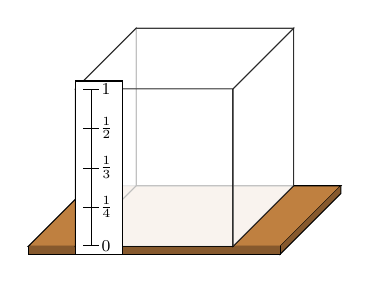
\begin{tikzpicture}[scale=2, x=1cm, y=1cm]

\draw [fill=brown] (-.3,0,0) -- (1.3,0,0) -- (1.3,0,1) -- (-.3,0,1) -- cycle;
\draw [fill=brown!70!black] (1.3,0,-0) -- (1.3,-.05,0) -- (1.3,-.05,1) -- (1.3,0,1);
\draw [fill=brown!70!black] (1.3,0,1) -- (1.3,-.05,1) -- (-.3,-.05,1) -- (-.3,0,1);



\draw [fill=white, opacity=.7] (0,0,0) -- (1,0,0) -- (1,0,1) -- (0,0,1) -- cycle;
\draw [fill=white, opacity=.7] (0,0,0) -- (0,1,0) -- (1,1,0) -- (1,0,0) -- cycle;
\draw [fill=white, opacity=.7] (0,0,0) -- (0,1,0) -- (0,1,1) -- (0,0,1) -- cycle;
\draw [fill=white, opacity=.7] (0,0,1) -- (1,0,1) -- (1,1,1) -- (0,1,1) -- cycle;
\draw [fill=white, opacity=.7] (1,0,0) -- (1,0,1) -- (1,1,1) -- (1,1,0) -- cycle;
\draw [fill=white, opacity=.7] (0,1,0) -- (1,1,0) -- (1,1,1) -- (0,1,1) -- cycle;

\filldraw [fill=white] (0,-.05,1) rectangle (0.3,1.05,1);
\draw [|-|] (.1,0,1) -- (.1,1,1) node [right, scale=.75, xshift=.05cm] {\footnotesize 1} node [ right, pos=0, scale=.75, xshift=.05cm]{\footnotesize 0};
\draw [|-|] (.1,0,1) -- (.1,.5,1) node [right, scale=.75, xshift=.025cm] {\footnotesize $\frac{1}{3}$};
\draw [|-|] (.1,0,1) -- (.1,.25,1) node [right, scale=.75, xshift=.025cm] {\footnotesize $\frac{1}{4}$};
\draw [|-|] (.1,0,1) -- (.1,.75,1) node [right, scale=.75, xshift=.025cm] { \footnotesize $\frac{1}{2}$};


\end{tikzpicture}
}
\end{multicols}

\begin{multicols}{2}

\item\adjustbox{valign=t}{
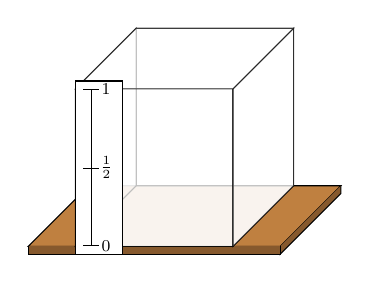
\begin{tikzpicture}[scale=2, x=1cm, y=1cm]

\draw [fill=brown] (-.3,0,0) -- (1.3,0,0) -- (1.3,0,1) -- (-.3,0,1) -- cycle;
\draw [fill=brown!70!black] (1.3,0,-0) -- (1.3,-.05,0) -- (1.3,-.05,1) -- (1.3,0,1);
\draw [fill=brown!70!black] (1.3,0,1) -- (1.3,-.05,1) -- (-.3,-.05,1) -- (-.3,0,1);


\draw [fill=white, opacity=.7] (0,0,0) -- (1,0,0) -- (1,0,1) -- (0,0,1) -- cycle;
\draw [fill=white, opacity=.7] (0,0,0) -- (0,1,0) -- (1,1,0) -- (1,0,0) -- cycle;
\draw [fill=white, opacity=.7] (0,0,0) -- (0,1,0) -- (0,1,1) -- (0,0,1) -- cycle;
\draw [fill=white, opacity=.7] (0,0,1) -- (1,0,1) -- (1,1,1) -- (0,1,1) -- cycle;
\draw [fill=white, opacity=.7] (1,0,0) -- (1,0,1) -- (1,1,1) -- (1,1,0) -- cycle;
\draw [fill=white, opacity=.7] (0,1,0) -- (1,1,0) -- (1,1,1) -- (0,1,1) -- cycle;

\filldraw [fill=white] (0,-.05,1) rectangle (0.3,1.05,1);
\draw [|-|] (.1,0,1) -- (.1,1,1) node [right, scale=.75, xshift=.05cm] {\footnotesize 1} node [ right, pos=0, scale=.75, xshift=.05cm]{\footnotesize 0};
\draw [|-|] (.1,0,1) -- (.1,.5,1) node [right, scale=.75, xshift=.025cm] {\footnotesize $\frac{1}{2}$};



\end{tikzpicture}


}
\end{multicols}
\end{enumerate}

\ifdefined\prof
\begin{solucao}

A faixa graduada b) é a mais indicada para registrar as quantidades de todos os momentos porque possui marcações com mesmo espaçamento, na ordem adequada e com informações claras para os quatro momentos. A graduação e), ainda que correta, só permite a leitura da quantidade de água nos momentos 2 e 4. Já a graduação a) tem a marcação $\frac{1}{2}$ associada ao segmento e não à um ponto, o que dificulta leituras intermediárias. A graduação c) não respeita a equipartição porque possui a marca $\frac{1}{2}$ em um ponto acima da metade da altura da caixa. Já na faixa graduada d) as marcações não respeitam a ordem, a marca $\frac{1}{2}$ é alcançada antes da marca $\frac{1}{3}$. 

\end{solucao}
\fi

\end{document}